\documentclass[12pt]{article}

%paquetes del idioma y codificacion
\usepackage[spanish,es-tabla]{babel}
\usepackage[utf8]{inputenc}
\usepackage[T1]{fontenc}
\usepackage{bookman}

%paquetes matematicos
\usepackage{amsmath, amsfonts, amssymb}

\usepackage{multirow}
\usepackage{float}
\usepackage{graphicx}

%dimensiones
\usepackage[left=2.5cm, right=2.5cm, top=1.5cm]{geometry}

\title{Tabla de conversión de un DFA a un NFA}
\author{Ian Mendoza Jaimes}
\date{}

\begin{document}

\maketitle
\begin{center}
\large
2CM4

Teoría Computacional 

Profesor Genaro Juárez Martínez
\end{center}

\vspace{6em}

Siempre es posible convertir un Autómata Finito No Determinístico (NFA) en uno Determinístico (DFA). Para este problema, el NFA es: y los subconjuntos que lo vuelven deterministico se muestran en la tabla \ref{tabla:conjuntos}, mientras que los conjuntos reducidos se muestran en la tabla \ref{tabla:conjuntos_renombrados}.\\

\begin{table}[H]
\centering
\begin{tabular}{|c|c|c|c|c|c|c|}
\hline 
\rule[-1ex]{0pt}{2.5ex}  & $\sum$ & w & e & b & a & y \\ 
\hline 
\rule[-1ex]{0pt}{2.5ex} $\emptyset$ & $\emptyset$ & $\emptyset$ & $\emptyset$ & $\emptyset$ & $\emptyset$ & $\emptyset$ \\ 
\hline 
\rule[-1ex]{0pt}{2.5ex} $\rightarrow\lbrace q_{0} \rbrace$ & $\lbrace q_{0} \rbrace$ & $\lbrace q_{0}, q_{1} \rbrace$ & $\lbrace q_{0}, q_{4} \rbrace$ & $\lbrace q_{0} \rbrace$ & $\lbrace q_{0} \rbrace$ & $\lbrace q_{0} \rbrace$ \\ 
\hline 
\rule[-1ex]{0pt}{2.5ex} $\lbrace q_{0}, q_{1} \rbrace$ & $\lbrace q_{0} \rbrace$ & $\lbrace q_{0}, q_{1} \rbrace$ & $\lbrace q_{0}, q_{2}, q_{4} \rbrace$ & $\lbrace q_{0} \rbrace$ & $\lbrace q_{0} \rbrace$ & $\lbrace q_{0} \rbrace$ \\ 
\hline 
\rule[-1ex]{0pt}{2.5ex} $\lbrace q_{0}, q_{4} \rbrace$ & $\lbrace q_{0} \rbrace$ & $\lbrace q_{0}, q_{1} \rbrace$ & $\lbrace q_{0}, q_{4} \rbrace$ & $\lbrace q_{0}, q_{5} \rbrace$ & $\lbrace q_{0} \rbrace$ & $\lbrace q_{0} \rbrace$ \\ 
\hline 
\rule[-1ex]{0pt}{2.5ex} $\lbrace q_{0}, q_{2}, q_{4} \rbrace$ & $\lbrace q_{0} \rbrace$ & $\lbrace q_{0}, q_{1} \rbrace$ & $\lbrace q_{0}, q_{4} \rbrace$ & $\lbrace q_{0}, q_{3}, q_{5} \rbrace$ & $\lbrace q_{0} \rbrace$ & $\lbrace q_{0} \rbrace$ \\ 
\hline 
\rule[-1ex]{0pt}{2.5ex} $\lbrace q_{0}, q_{5} \rbrace$ & $\lbrace q_{0} \rbrace$ & $\lbrace q_{0}, q_{1} \rbrace$ & $\lbrace q_{0}, q_{4} \rbrace$ & $\lbrace q_{0} \rbrace$ & $\lbrace q_{0}, q_{6} \rbrace$ & $\lbrace q_{0} \rbrace$ \\ 
\hline 
\rule[-1ex]{0pt}{2.5ex} $* \lbrace q_{0}, q_{3}, q_{5} \rbrace$ & $\lbrace q_{0} \rbrace$ & $\lbrace q_{0}, q_{1} \rbrace$ & $\lbrace q_{0}, q_{4} \rbrace$ & $\lbrace q_{0} \rbrace$ & $\lbrace q_{0}, q_{6} \rbrace$ & $\lbrace q_{0} \rbrace$ \\ 
\hline 
\rule[-1ex]{0pt}{2.5ex} $\lbrace q_{0}, q_{6} \rbrace$ & $\lbrace q_{0} \rbrace$ & $\lbrace q_{0}, q_{1} \rbrace$ & $\lbrace q_{0}, q_{4} \rbrace$ & $\lbrace q_{0} \rbrace$ & $\lbrace q_{0} \rbrace$ & $\lbrace q_{0}, q_{7} \rbrace$ \\ 
\hline 
\rule[-1ex]{0pt}{2.5ex} $* \lbrace q_{0}, q_{7} \rbrace$ & $\lbrace q_{0} \rbrace$ & $\lbrace q_{0}, q_{1} \rbrace$ & $\lbrace q_{0}, q_{4} \rbrace$ & $\lbrace q_{0} \rbrace$ & $\lbrace q_{0} \rbrace$ & $\lbrace q_{0} \rbrace$ \\ 
\hline 
\end{tabular} 
\caption{Conjuntos que vuelven DFA a este NFA.}
\label{tabla:conjuntos}
\end{table}


\vspace{2em}

\begin{table}[H]
\centering
\begin{tabular}{|c|c|c|c|c|c|c|}
\hline 
\rule[-1ex]{0pt}{2.5ex}  & $\sum$ & w & e & b & a & y \\ 
\hline 
\rule[-1ex]{0pt}{2.5ex} A & A & A & A & A & A & A \\ 
\hline 
\rule[-1ex]{0pt}{2.5ex} $\rightarrow$B & B & C & D & B & B & B \\ 
\hline 
\rule[-1ex]{0pt}{2.5ex} C & B & C & E & B & B & B \\ 
\hline 
\rule[-1ex]{0pt}{2.5ex} D & B & C & D & F & B & B \\ 
\hline 
\rule[-1ex]{0pt}{2.5ex} E & B & C & D & G & B & B \\ 
\hline 
\rule[-1ex]{0pt}{2.5ex} F & B & C & D & B & H & B \\ 
\hline 
\rule[-1ex]{0pt}{2.5ex} *G & B & C & D & B & H & B \\ 
\hline 
\rule[-1ex]{0pt}{2.5ex} H & B & C & D & B & B & I \\ 
\hline 
\rule[-1ex]{0pt}{2.5ex} *I & B & C & D & B & B & B \\ 
\hline 
\end{tabular}
\caption{Conjuntos renombrados.}
\label{tabla:conjuntos_renombrados}
\end{table}

\vspace{1em}

El correspondiente DFA obtenido a partir de la tabla \ref{tabla:conjuntos_renombrados} es el siguiente:

\begin{figure}[H]
\centering
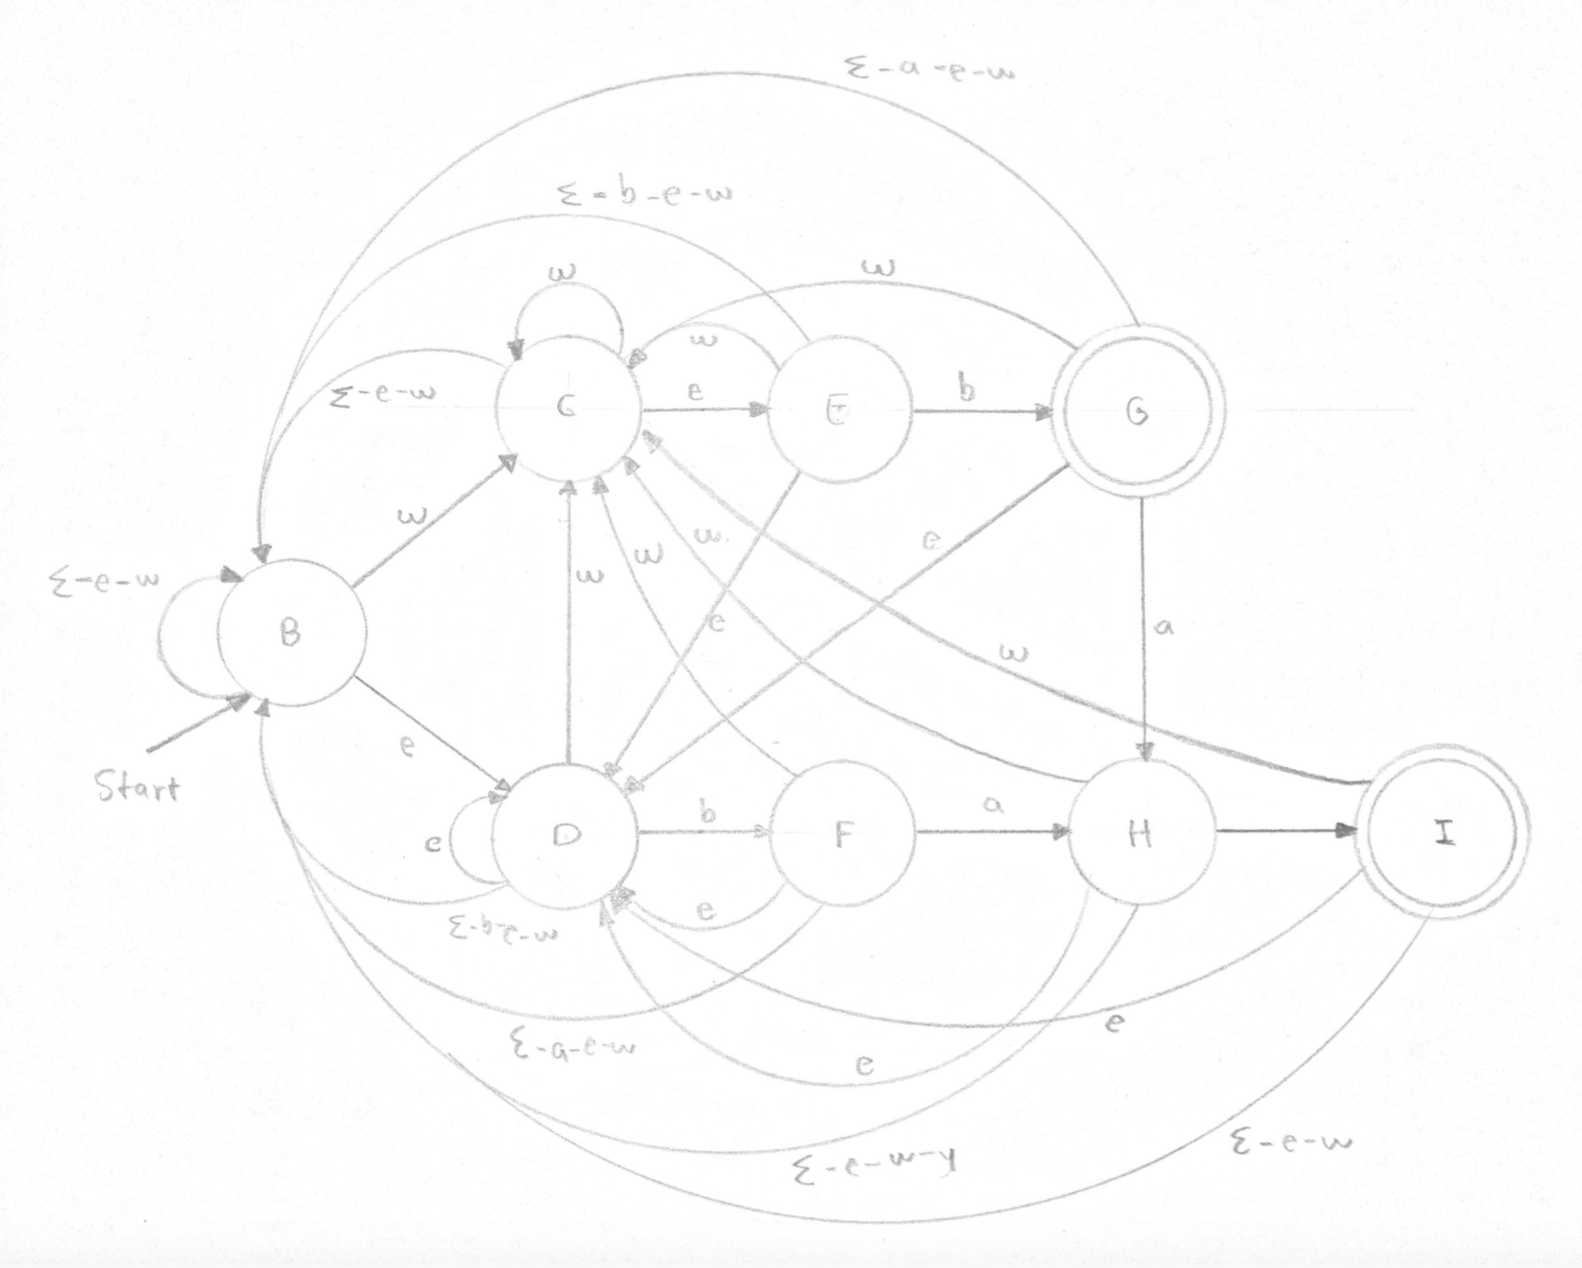
\includegraphics[width=\textwidth, height=13cm]{automata}
\caption{NFA convertido a DFA.}
\label{figura:automata}
\end{figure}

\end{document}